% Created by tikzDevice version 0.12.6 on 2026-08-02 12:20:24
% !TEX encoding = UTF-8 Unicode
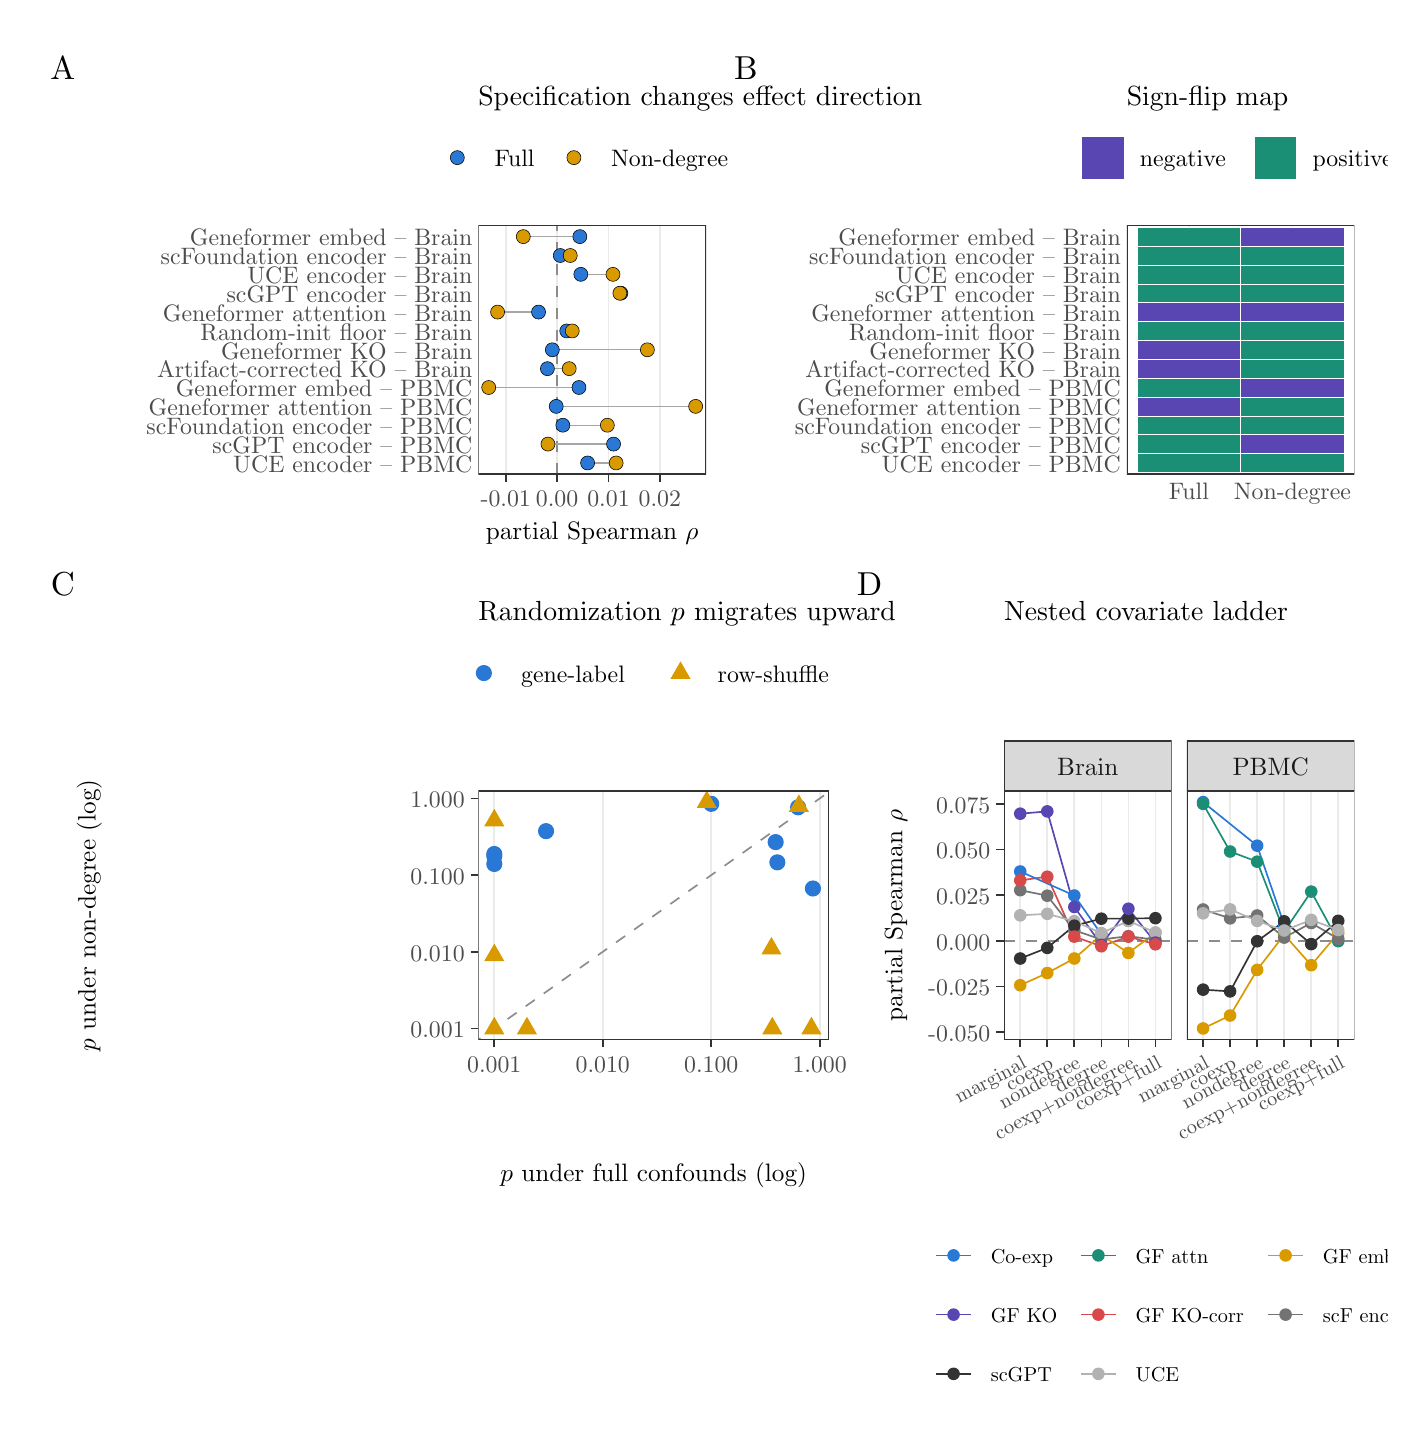
\begin{tikzpicture}[x=1pt,y=1pt]
\definecolor{fillColor}{RGB}{255,255,255}
\path[use as bounding box,fill=fillColor,fill opacity=0.00] (0,0) rectangle (491.44,505.89);
\begin{scope}
\path[clip] (  0.00,  0.00) rectangle (491.44,505.89);
\definecolor{drawColor}{RGB}{255,255,255}
\definecolor{fillColor}{RGB}{255,255,255}

\path[draw=drawColor,line width= 0.6pt,line join=round,line cap=round,fill=fillColor] (  0.00, -0.00) rectangle (491.44,505.89);
\end{scope}
\begin{scope}
\path[clip] (  4.00,315.66) rectangle (251.11,501.89);
\definecolor{drawColor}{RGB}{255,255,255}
\definecolor{fillColor}{RGB}{255,255,255}

\path[draw=drawColor,line width= 0.6pt,line join=round,line cap=round,fill=fillColor] (  4.00,315.66) rectangle (251.11,501.89);
\end{scope}
\begin{scope}
\path[clip] (251.11,315.66) rectangle (485.44,501.89);
\definecolor{drawColor}{RGB}{255,255,255}
\definecolor{fillColor}{RGB}{255,255,255}

\path[draw=drawColor,line width= 0.6pt,line join=round,line cap=round,fill=fillColor] (251.11,315.66) rectangle (485.44,501.89);
\end{scope}
\begin{scope}
\path[clip] (162.86,344.51) rectangle (245.11,434.47);
\definecolor{fillColor}{RGB}{255,255,255}

\path[fill=fillColor] (162.86,344.51) rectangle (245.11,434.47);
\definecolor{drawColor}{gray}{0.92}

\path[draw=drawColor,line width= 0.6pt,line join=round] (172.75,344.51) --
	(172.75,434.47);

\path[draw=drawColor,line width= 0.6pt,line join=round] (191.32,344.51) --
	(191.32,434.47);

\path[draw=drawColor,line width= 0.6pt,line join=round] (209.88,344.51) --
	(209.88,434.47);

\path[draw=drawColor,line width= 0.6pt,line join=round] (228.44,344.51) --
	(228.44,434.47);
\definecolor{drawColor}{gray}{0.55}

\path[draw=drawColor,line width= 0.6pt,dash pattern=on 4pt off 4pt ,line join=round] (191.32,344.51) -- (191.32,434.47);
\definecolor{drawColor}{gray}{0.65}

\path[draw=drawColor,line width= 0.5pt,line join=round] (202.32,348.59) --
	(212.64,348.59);

\path[draw=drawColor,line width= 0.5pt,line join=round] (188.00,355.41) --
	(211.70,355.41);

\path[draw=drawColor,line width= 0.5pt,line join=round] (193.39,362.23) --
	(209.46,362.23);

\path[draw=drawColor,line width= 0.5pt,line join=round] (190.99,369.04) --
	(241.37,369.04);

\path[draw=drawColor,line width= 0.5pt,line join=round] (166.60,375.86) --
	(199.21,375.86);

\path[draw=drawColor,line width= 0.5pt,line join=round] (187.81,382.67) --
	(195.68,382.67);

\path[draw=drawColor,line width= 0.5pt,line join=round] (189.58,389.49) --
	(223.93,389.49);

\path[draw=drawColor,line width= 0.5pt,line join=round] (194.79,396.30) --
	(196.78,396.30);

\path[draw=drawColor,line width= 0.5pt,line join=round] (169.80,403.12) --
	(184.60,403.12);

\path[draw=drawColor,line width= 0.5pt,line join=round] (213.99,409.93) --
	(214.35,409.93);

\path[draw=drawColor,line width= 0.5pt,line join=round] (199.88,416.75) --
	(211.50,416.75);

\path[draw=drawColor,line width= 0.5pt,line join=round] (192.46,423.56) --
	(196.06,423.56);

\path[draw=drawColor,line width= 0.5pt,line join=round] (179.09,430.38) --
	(199.52,430.38);
\definecolor{drawColor}{RGB}{0,0,0}
\definecolor{fillColor}{RGB}{42,120,214}

\path[draw=drawColor,line width= 0.2pt,line join=round,line cap=round,fill=fillColor] (199.52,430.38) circle (  2.53);
\definecolor{fillColor}{RGB}{217,154,0}

\path[draw=drawColor,line width= 0.2pt,line join=round,line cap=round,fill=fillColor] (179.09,430.38) circle (  2.53);
\definecolor{fillColor}{RGB}{42,120,214}

\path[draw=drawColor,line width= 0.2pt,line join=round,line cap=round,fill=fillColor] (192.46,423.56) circle (  2.53);
\definecolor{fillColor}{RGB}{217,154,0}

\path[draw=drawColor,line width= 0.2pt,line join=round,line cap=round,fill=fillColor] (196.06,423.56) circle (  2.53);
\definecolor{fillColor}{RGB}{42,120,214}

\path[draw=drawColor,line width= 0.2pt,line join=round,line cap=round,fill=fillColor] (199.88,416.75) circle (  2.53);
\definecolor{fillColor}{RGB}{217,154,0}

\path[draw=drawColor,line width= 0.2pt,line join=round,line cap=round,fill=fillColor] (211.50,416.75) circle (  2.53);
\definecolor{fillColor}{RGB}{42,120,214}

\path[draw=drawColor,line width= 0.2pt,line join=round,line cap=round,fill=fillColor] (214.35,409.93) circle (  2.53);
\definecolor{fillColor}{RGB}{217,154,0}

\path[draw=drawColor,line width= 0.2pt,line join=round,line cap=round,fill=fillColor] (213.99,409.93) circle (  2.53);
\definecolor{fillColor}{RGB}{42,120,214}

\path[draw=drawColor,line width= 0.2pt,line join=round,line cap=round,fill=fillColor] (184.60,403.12) circle (  2.53);
\definecolor{fillColor}{RGB}{217,154,0}

\path[draw=drawColor,line width= 0.2pt,line join=round,line cap=round,fill=fillColor] (169.80,403.12) circle (  2.53);
\definecolor{fillColor}{RGB}{42,120,214}

\path[draw=drawColor,line width= 0.2pt,line join=round,line cap=round,fill=fillColor] (194.79,396.30) circle (  2.53);
\definecolor{fillColor}{RGB}{217,154,0}

\path[draw=drawColor,line width= 0.2pt,line join=round,line cap=round,fill=fillColor] (196.78,396.30) circle (  2.53);
\definecolor{fillColor}{RGB}{42,120,214}

\path[draw=drawColor,line width= 0.2pt,line join=round,line cap=round,fill=fillColor] (189.58,389.49) circle (  2.53);
\definecolor{fillColor}{RGB}{217,154,0}

\path[draw=drawColor,line width= 0.2pt,line join=round,line cap=round,fill=fillColor] (223.93,389.49) circle (  2.53);
\definecolor{fillColor}{RGB}{42,120,214}

\path[draw=drawColor,line width= 0.2pt,line join=round,line cap=round,fill=fillColor] (187.81,382.67) circle (  2.53);
\definecolor{fillColor}{RGB}{217,154,0}

\path[draw=drawColor,line width= 0.2pt,line join=round,line cap=round,fill=fillColor] (195.68,382.67) circle (  2.53);
\definecolor{fillColor}{RGB}{42,120,214}

\path[draw=drawColor,line width= 0.2pt,line join=round,line cap=round,fill=fillColor] (199.21,375.86) circle (  2.53);
\definecolor{fillColor}{RGB}{217,154,0}

\path[draw=drawColor,line width= 0.2pt,line join=round,line cap=round,fill=fillColor] (166.60,375.86) circle (  2.53);
\definecolor{fillColor}{RGB}{42,120,214}

\path[draw=drawColor,line width= 0.2pt,line join=round,line cap=round,fill=fillColor] (190.99,369.04) circle (  2.53);
\definecolor{fillColor}{RGB}{217,154,0}

\path[draw=drawColor,line width= 0.2pt,line join=round,line cap=round,fill=fillColor] (241.37,369.04) circle (  2.53);
\definecolor{fillColor}{RGB}{42,120,214}

\path[draw=drawColor,line width= 0.2pt,line join=round,line cap=round,fill=fillColor] (193.39,362.23) circle (  2.53);
\definecolor{fillColor}{RGB}{217,154,0}

\path[draw=drawColor,line width= 0.2pt,line join=round,line cap=round,fill=fillColor] (209.46,362.23) circle (  2.53);
\definecolor{fillColor}{RGB}{42,120,214}

\path[draw=drawColor,line width= 0.2pt,line join=round,line cap=round,fill=fillColor] (211.70,355.41) circle (  2.53);
\definecolor{fillColor}{RGB}{217,154,0}

\path[draw=drawColor,line width= 0.2pt,line join=round,line cap=round,fill=fillColor] (188.00,355.41) circle (  2.53);
\definecolor{fillColor}{RGB}{42,120,214}

\path[draw=drawColor,line width= 0.2pt,line join=round,line cap=round,fill=fillColor] (202.32,348.59) circle (  2.53);
\definecolor{fillColor}{RGB}{217,154,0}

\path[draw=drawColor,line width= 0.2pt,line join=round,line cap=round,fill=fillColor] (212.64,348.59) circle (  2.53);
\definecolor{drawColor}{gray}{0.20}

\path[draw=drawColor,line width= 0.6pt,line join=round,line cap=round] (162.86,344.51) rectangle (245.11,434.47);
\end{scope}
\begin{scope}
\path[clip] (  0.00,  0.00) rectangle (491.44,505.89);
\definecolor{drawColor}{gray}{0.30}

\node[text=drawColor,anchor=base east,inner sep=0pt, outer sep=0pt, scale=  0.86] at (160.66,345.23) {UCE encoder -- PBMC};

\node[text=drawColor,anchor=base east,inner sep=0pt, outer sep=0pt, scale=  0.86] at (160.66,352.04) {scGPT encoder -- PBMC};

\node[text=drawColor,anchor=base east,inner sep=0pt, outer sep=0pt, scale=  0.86] at (160.66,358.86) {scFoundation encoder -- PBMC};

\node[text=drawColor,anchor=base east,inner sep=0pt, outer sep=0pt, scale=  0.86] at (160.66,365.67) {Geneformer attention -- PBMC};

\node[text=drawColor,anchor=base east,inner sep=0pt, outer sep=0pt, scale=  0.86] at (160.66,372.49) {Geneformer embed -- PBMC};

\node[text=drawColor,anchor=base east,inner sep=0pt, outer sep=0pt, scale=  0.86] at (160.66,379.30) {Artifact-corrected KO -- Brain};

\node[text=drawColor,anchor=base east,inner sep=0pt, outer sep=0pt, scale=  0.86] at (160.66,386.12) {Geneformer KO -- Brain};

\node[text=drawColor,anchor=base east,inner sep=0pt, outer sep=0pt, scale=  0.86] at (160.66,392.93) {Random-init floor -- Brain};

\node[text=drawColor,anchor=base east,inner sep=0pt, outer sep=0pt, scale=  0.86] at (160.66,399.75) {Geneformer attention -- Brain};

\node[text=drawColor,anchor=base east,inner sep=0pt, outer sep=0pt, scale=  0.86] at (160.66,406.56) {scGPT encoder -- Brain};

\node[text=drawColor,anchor=base east,inner sep=0pt, outer sep=0pt, scale=  0.86] at (160.66,413.38) {UCE encoder -- Brain};

\node[text=drawColor,anchor=base east,inner sep=0pt, outer sep=0pt, scale=  0.86] at (160.66,420.19) {scFoundation encoder -- Brain};

\node[text=drawColor,anchor=base east,inner sep=0pt, outer sep=0pt, scale=  0.86] at (160.66,427.01) {Geneformer embed -- Brain};
\end{scope}
\begin{scope}
\path[clip] (  0.00,  0.00) rectangle (491.44,505.89);
\definecolor{drawColor}{gray}{0.20}

\path[draw=drawColor,line width= 0.6pt,line join=round] (172.75,341.76) --
	(172.75,344.51);

\path[draw=drawColor,line width= 0.6pt,line join=round] (191.32,341.76) --
	(191.32,344.51);

\path[draw=drawColor,line width= 0.6pt,line join=round] (209.88,341.76) --
	(209.88,344.51);

\path[draw=drawColor,line width= 0.6pt,line join=round] (228.44,341.76) --
	(228.44,344.51);
\end{scope}
\begin{scope}
\path[clip] (  0.00,  0.00) rectangle (491.44,505.89);
\definecolor{drawColor}{gray}{0.30}

\node[text=drawColor,anchor=base,inner sep=0pt, outer sep=0pt, scale=  0.86] at (172.75,332.82) {-0.01};

\node[text=drawColor,anchor=base,inner sep=0pt, outer sep=0pt, scale=  0.86] at (191.32,332.82) {0.00};

\node[text=drawColor,anchor=base,inner sep=0pt, outer sep=0pt, scale=  0.86] at (209.88,332.82) {0.01};

\node[text=drawColor,anchor=base,inner sep=0pt, outer sep=0pt, scale=  0.86] at (228.44,332.82) {0.02};
\end{scope}
\begin{scope}
\path[clip] (  0.00,  0.00) rectangle (491.44,505.89);
\definecolor{drawColor}{RGB}{0,0,0}

\node[text=drawColor,anchor=base,inner sep=0pt, outer sep=0pt, scale=  0.91] at (203.98,320.87) {partial Spearman $\rho$};
\end{scope}
\begin{scope}
\path[clip] (  0.00,  0.00) rectangle (491.44,505.89);
\definecolor{fillColor}{RGB}{255,255,255}

\path[fill=fillColor] (141.80,445.47) rectangle (266.17,472.37);
\end{scope}
\begin{scope}
\path[clip] (  0.00,  0.00) rectangle (491.44,505.89);
\definecolor{fillColor}{RGB}{255,255,255}

\path[fill=fillColor] (147.30,450.97) rectangle (163.20,466.87);
\definecolor{drawColor}{RGB}{0,0,0}
\definecolor{fillColor}{RGB}{42,120,214}

\path[draw=drawColor,line width= 0.2pt,line join=round,line cap=round,fill=fillColor] (155.25,458.92) circle (  2.53);
\end{scope}
\begin{scope}
\path[clip] (  0.00,  0.00) rectangle (491.44,505.89);
\definecolor{fillColor}{RGB}{255,255,255}

\path[fill=fillColor] (189.43,450.97) rectangle (205.33,466.87);
\definecolor{drawColor}{RGB}{0,0,0}
\definecolor{fillColor}{RGB}{217,154,0}

\path[draw=drawColor,line width= 0.2pt,line join=round,line cap=round,fill=fillColor] (197.38,458.92) circle (  2.53);
\end{scope}
\begin{scope}
\path[clip] (  0.00,  0.00) rectangle (491.44,505.89);
\definecolor{drawColor}{RGB}{0,0,0}

\node[text=drawColor,anchor=base west,inner sep=0pt, outer sep=0pt, scale=  0.86] at (168.70,455.55) {Full};
\end{scope}
\begin{scope}
\path[clip] (  0.00,  0.00) rectangle (491.44,505.89);
\definecolor{drawColor}{RGB}{0,0,0}

\node[text=drawColor,anchor=base west,inner sep=0pt, outer sep=0pt, scale=  0.86] at (210.83,455.55) {Non-degree};
\end{scope}
\begin{scope}
\path[clip] (  0.00,  0.00) rectangle (491.44,505.89);
\definecolor{drawColor}{RGB}{0,0,0}

\node[text=drawColor,anchor=base west,inner sep=0pt, outer sep=0pt, scale=  1.00] at (162.86,477.80) {Specification changes effect direction};
\end{scope}
\begin{scope}
\path[clip] (  0.00,  0.00) rectangle (491.44,505.89);
\definecolor{drawColor}{RGB}{0,0,0}

\node[text=drawColor,anchor=base,inner sep=0pt, outer sep=0pt, scale=  1.20] at ( 12.74,487.07) {A};
\end{scope}
\begin{scope}
\path[clip] (397.18,344.51) rectangle (479.44,434.47);
\definecolor{fillColor}{RGB}{255,255,255}

\path[fill=fillColor] (397.18,344.51) rectangle (479.44,434.47);
\definecolor{drawColor}{gray}{0.92}

\path[draw=drawColor,line width= 0.6pt,line join=round] (419.62,344.51) --
	(419.62,434.47);

\path[draw=drawColor,line width= 0.6pt,line join=round] (457.00,344.51) --
	(457.00,434.47);
\definecolor{drawColor}{RGB}{255,255,255}
\definecolor{fillColor}{RGB}{27,143,117}

\path[draw=drawColor,line width= 0.2pt,fill=fillColor] (400.92,426.97) rectangle (438.31,433.79);
\definecolor{fillColor}{RGB}{89,70,178}

\path[draw=drawColor,line width= 0.2pt,fill=fillColor] (438.31,426.97) rectangle (475.70,433.79);
\definecolor{fillColor}{RGB}{27,143,117}

\path[draw=drawColor,line width= 0.2pt,fill=fillColor] (400.92,420.15) rectangle (438.31,426.97);

\path[draw=drawColor,line width= 0.2pt,fill=fillColor] (438.31,420.15) rectangle (475.70,426.97);

\path[draw=drawColor,line width= 0.2pt,fill=fillColor] (400.92,413.34) rectangle (438.31,420.15);

\path[draw=drawColor,line width= 0.2pt,fill=fillColor] (438.31,413.34) rectangle (475.70,420.15);

\path[draw=drawColor,line width= 0.2pt,fill=fillColor] (400.92,406.52) rectangle (438.31,413.34);

\path[draw=drawColor,line width= 0.2pt,fill=fillColor] (438.31,406.52) rectangle (475.70,413.34);
\definecolor{fillColor}{RGB}{89,70,178}

\path[draw=drawColor,line width= 0.2pt,fill=fillColor] (400.92,399.71) rectangle (438.31,406.52);

\path[draw=drawColor,line width= 0.2pt,fill=fillColor] (438.31,399.71) rectangle (475.70,406.52);
\definecolor{fillColor}{RGB}{27,143,117}

\path[draw=drawColor,line width= 0.2pt,fill=fillColor] (400.92,392.89) rectangle (438.31,399.71);

\path[draw=drawColor,line width= 0.2pt,fill=fillColor] (438.31,392.89) rectangle (475.70,399.71);
\definecolor{fillColor}{RGB}{89,70,178}

\path[draw=drawColor,line width= 0.2pt,fill=fillColor] (400.92,386.08) rectangle (438.31,392.89);
\definecolor{fillColor}{RGB}{27,143,117}

\path[draw=drawColor,line width= 0.2pt,fill=fillColor] (438.31,386.08) rectangle (475.70,392.89);
\definecolor{fillColor}{RGB}{89,70,178}

\path[draw=drawColor,line width= 0.2pt,fill=fillColor] (400.92,379.26) rectangle (438.31,386.08);
\definecolor{fillColor}{RGB}{27,143,117}

\path[draw=drawColor,line width= 0.2pt,fill=fillColor] (438.31,379.26) rectangle (475.70,386.08);

\path[draw=drawColor,line width= 0.2pt,fill=fillColor] (400.92,372.45) rectangle (438.31,379.26);
\definecolor{fillColor}{RGB}{89,70,178}

\path[draw=drawColor,line width= 0.2pt,fill=fillColor] (438.31,372.45) rectangle (475.70,379.26);

\path[draw=drawColor,line width= 0.2pt,fill=fillColor] (400.92,365.63) rectangle (438.31,372.45);
\definecolor{fillColor}{RGB}{27,143,117}

\path[draw=drawColor,line width= 0.2pt,fill=fillColor] (438.31,365.63) rectangle (475.70,372.45);

\path[draw=drawColor,line width= 0.2pt,fill=fillColor] (400.92,358.82) rectangle (438.31,365.63);

\path[draw=drawColor,line width= 0.2pt,fill=fillColor] (438.31,358.82) rectangle (475.70,365.63);

\path[draw=drawColor,line width= 0.2pt,fill=fillColor] (400.92,352.00) rectangle (438.31,358.82);
\definecolor{fillColor}{RGB}{89,70,178}

\path[draw=drawColor,line width= 0.2pt,fill=fillColor] (438.31,352.00) rectangle (475.70,358.82);
\definecolor{fillColor}{RGB}{27,143,117}

\path[draw=drawColor,line width= 0.2pt,fill=fillColor] (400.92,345.19) rectangle (438.31,352.00);

\path[draw=drawColor,line width= 0.2pt,fill=fillColor] (438.31,345.19) rectangle (475.70,352.00);
\definecolor{drawColor}{gray}{0.20}

\path[draw=drawColor,line width= 0.6pt,line join=round,line cap=round] (397.18,344.51) rectangle (479.44,434.47);
\end{scope}
\begin{scope}
\path[clip] (  0.00,  0.00) rectangle (491.44,505.89);
\definecolor{drawColor}{gray}{0.30}

\node[text=drawColor,anchor=base east,inner sep=0pt, outer sep=0pt, scale=  0.86] at (394.98,345.23) {UCE encoder -- PBMC};

\node[text=drawColor,anchor=base east,inner sep=0pt, outer sep=0pt, scale=  0.86] at (394.98,352.04) {scGPT encoder -- PBMC};

\node[text=drawColor,anchor=base east,inner sep=0pt, outer sep=0pt, scale=  0.86] at (394.98,358.86) {scFoundation encoder -- PBMC};

\node[text=drawColor,anchor=base east,inner sep=0pt, outer sep=0pt, scale=  0.86] at (394.98,365.67) {Geneformer attention -- PBMC};

\node[text=drawColor,anchor=base east,inner sep=0pt, outer sep=0pt, scale=  0.86] at (394.98,372.49) {Geneformer embed -- PBMC};

\node[text=drawColor,anchor=base east,inner sep=0pt, outer sep=0pt, scale=  0.86] at (394.98,379.30) {Artifact-corrected KO -- Brain};

\node[text=drawColor,anchor=base east,inner sep=0pt, outer sep=0pt, scale=  0.86] at (394.98,386.12) {Geneformer KO -- Brain};

\node[text=drawColor,anchor=base east,inner sep=0pt, outer sep=0pt, scale=  0.86] at (394.98,392.93) {Random-init floor -- Brain};

\node[text=drawColor,anchor=base east,inner sep=0pt, outer sep=0pt, scale=  0.86] at (394.98,399.75) {Geneformer attention -- Brain};

\node[text=drawColor,anchor=base east,inner sep=0pt, outer sep=0pt, scale=  0.86] at (394.98,406.56) {scGPT encoder -- Brain};

\node[text=drawColor,anchor=base east,inner sep=0pt, outer sep=0pt, scale=  0.86] at (394.98,413.38) {UCE encoder -- Brain};

\node[text=drawColor,anchor=base east,inner sep=0pt, outer sep=0pt, scale=  0.86] at (394.98,420.19) {scFoundation encoder -- Brain};

\node[text=drawColor,anchor=base east,inner sep=0pt, outer sep=0pt, scale=  0.86] at (394.98,427.01) {Geneformer embed -- Brain};
\end{scope}
\begin{scope}
\path[clip] (  0.00,  0.00) rectangle (491.44,505.89);
\definecolor{drawColor}{gray}{0.30}

\node[text=drawColor,anchor=base,inner sep=0pt, outer sep=0pt, scale=  0.86] at (419.62,335.57) {Full};

\node[text=drawColor,anchor=base,inner sep=0pt, outer sep=0pt, scale=  0.86] at (457.00,335.57) {Non-degree};
\end{scope}
\begin{scope}
\path[clip] (  0.00,  0.00) rectangle (491.44,505.89);
\definecolor{fillColor}{RGB}{255,255,255}

\path[fill=fillColor] (375.00,445.47) rectangle (501.62,472.37);
\end{scope}
\begin{scope}
\path[clip] (  0.00,  0.00) rectangle (491.44,505.89);
\definecolor{fillColor}{RGB}{255,255,255}

\path[fill=fillColor] (380.50,450.97) rectangle (396.40,466.87);
\definecolor{drawColor}{RGB}{255,255,255}
\definecolor{fillColor}{RGB}{89,70,178}

\path[draw=drawColor,line width= 0.2pt,fill=fillColor] (380.78,451.25) rectangle (396.11,466.58);
\end{scope}
\begin{scope}
\path[clip] (  0.00,  0.00) rectangle (491.44,505.89);
\definecolor{fillColor}{RGB}{255,255,255}

\path[fill=fillColor] (442.90,450.97) rectangle (458.80,466.87);
\definecolor{drawColor}{RGB}{255,255,255}
\definecolor{fillColor}{RGB}{27,143,117}

\path[draw=drawColor,line width= 0.2pt,fill=fillColor] (443.19,451.25) rectangle (458.52,466.58);
\end{scope}
\begin{scope}
\path[clip] (  0.00,  0.00) rectangle (491.44,505.89);
\definecolor{drawColor}{RGB}{0,0,0}

\node[text=drawColor,anchor=base west,inner sep=0pt, outer sep=0pt, scale=  0.86] at (401.90,455.55) {negative};
\end{scope}
\begin{scope}
\path[clip] (  0.00,  0.00) rectangle (491.44,505.89);
\definecolor{drawColor}{RGB}{0,0,0}

\node[text=drawColor,anchor=base west,inner sep=0pt, outer sep=0pt, scale=  0.86] at (464.30,455.55) {positive};
\end{scope}
\begin{scope}
\path[clip] (  0.00,  0.00) rectangle (491.44,505.89);
\definecolor{drawColor}{RGB}{0,0,0}

\node[text=drawColor,anchor=base west,inner sep=0pt, outer sep=0pt, scale=  1.00] at (397.18,477.80) {Sign-flip map};
\end{scope}
\begin{scope}
\path[clip] (  0.00,  0.00) rectangle (491.44,505.89);
\definecolor{drawColor}{RGB}{0,0,0}

\node[text=drawColor,anchor=base,inner sep=0pt, outer sep=0pt, scale=  1.20] at (259.49,487.07) {B};
\end{scope}
\begin{scope}
\path[clip] (  4.00,  3.00) rectangle (295.49,315.66);
\definecolor{drawColor}{RGB}{255,255,255}
\definecolor{fillColor}{RGB}{255,255,255}

\path[draw=drawColor,line width= 0.6pt,line join=round,line cap=round,fill=fillColor] (  4.00,  3.00) rectangle (295.49,315.66);
\end{scope}
\begin{scope}
\path[clip] (295.49,  3.00) rectangle (485.44,315.66);
\definecolor{drawColor}{RGB}{255,255,255}
\definecolor{fillColor}{RGB}{255,255,255}

\path[draw=drawColor,line width= 0.6pt,line join=round,line cap=round,fill=fillColor] (295.49,  3.00) rectangle (485.44,315.66);
\end{scope}
\begin{scope}
\path[clip] (162.86,140.16) rectangle (289.49,230.13);
\definecolor{fillColor}{RGB}{255,255,255}

\path[fill=fillColor] (162.86,140.16) rectangle (289.49,230.13);
\definecolor{drawColor}{gray}{0.92}

\path[draw=drawColor,line width= 0.6pt,line join=round] (168.61,140.16) --
	(168.61,230.13);

\path[draw=drawColor,line width= 0.6pt,line join=round] (207.80,140.16) --
	(207.80,230.13);

\path[draw=drawColor,line width= 0.6pt,line join=round] (247.00,140.16) --
	(247.00,230.13);

\path[draw=drawColor,line width= 0.6pt,line join=round] (286.19,140.16) --
	(286.19,230.13);
\definecolor{drawColor}{gray}{0.55}

\path[draw=drawColor,line width= 0.6pt,dash pattern=on 4pt off 4pt ,line join=round] ( 36.22, 50.69) -- (416.13,319.18);
\definecolor{drawColor}{RGB}{42,120,214}
\definecolor{fillColor}{RGB}{42,120,214}

\path[draw=drawColor,line width= 0.4pt,line join=round,line cap=round,fill=fillColor] (187.31,215.55) circle (  2.71);

\path[draw=drawColor,line width= 0.4pt,line join=round,line cap=round,fill=fillColor] (278.40,224.17) circle (  2.71);

\path[draw=drawColor,line width= 0.4pt,line join=round,line cap=round,fill=fillColor] (168.61,203.69) circle (  2.71);

\path[draw=drawColor,line width= 0.4pt,line join=round,line cap=round,fill=fillColor] (168.61,206.52) circle (  2.71);

\path[draw=drawColor,line width= 0.4pt,line join=round,line cap=round,fill=fillColor] (270.89,204.28) circle (  2.71);

\path[draw=drawColor,line width= 0.4pt,line join=round,line cap=round,fill=fillColor] (247.00,225.42) circle (  2.71);

\path[draw=drawColor,line width= 0.4pt,line join=round,line cap=round,fill=fillColor] (168.61,207.30) circle (  2.71);

\path[draw=drawColor,line width= 0.4pt,line join=round,line cap=round,fill=fillColor] (283.74,194.83) circle (  2.71);

\path[draw=drawColor,line width= 0.4pt,line join=round,line cap=round,fill=fillColor] (270.29,211.59) circle (  2.71);
\definecolor{fillColor}{RGB}{217,154,0}

\path[fill=fillColor] (168.61,223.63) --
	(172.26,217.30) --
	(164.96,217.30) --
	cycle;

\path[fill=fillColor] (278.67,228.83) --
	(282.32,222.51) --
	(275.02,222.51) --
	cycle;

\path[fill=fillColor] (168.61,148.47) --
	(172.26,142.14) --
	(164.96,142.14) --
	cycle;

\path[fill=fillColor] (168.61,174.90) --
	(172.26,168.57) --
	(164.96,168.57) --
	cycle;

\path[fill=fillColor] (269.08,148.47) --
	(272.73,142.14) --
	(265.43,142.14) --
	cycle;

\path[fill=fillColor] (245.39,230.25) --
	(249.04,223.93) --
	(241.74,223.93) --
	cycle;

\path[fill=fillColor] (180.41,148.47) --
	(184.06,142.14) --
	(176.76,142.14) --
	cycle;

\path[fill=fillColor] (283.20,148.47) --
	(286.85,142.14) --
	(279.55,142.14) --
	cycle;

\path[fill=fillColor] (268.75,177.31) --
	(272.40,170.99) --
	(265.10,170.99) --
	cycle;
\definecolor{drawColor}{gray}{0.20}

\path[draw=drawColor,line width= 0.6pt,line join=round,line cap=round] (162.86,140.16) rectangle (289.49,230.13);
\end{scope}
\begin{scope}
\path[clip] (  0.00,  0.00) rectangle (491.44,505.89);
\definecolor{drawColor}{gray}{0.30}

\node[text=drawColor,anchor=base east,inner sep=0pt, outer sep=0pt, scale=  0.86] at (157.91,140.88) {0.001};

\node[text=drawColor,anchor=base east,inner sep=0pt, outer sep=0pt, scale=  0.86] at (157.91,168.58) {0.010};

\node[text=drawColor,anchor=base east,inner sep=0pt, outer sep=0pt, scale=  0.86] at (157.91,196.28) {0.100};

\node[text=drawColor,anchor=base east,inner sep=0pt, outer sep=0pt, scale=  0.86] at (157.91,223.98) {1.000};
\end{scope}
\begin{scope}
\path[clip] (  0.00,  0.00) rectangle (491.44,505.89);
\definecolor{drawColor}{gray}{0.20}

\path[draw=drawColor,line width= 0.6pt,line join=round] (160.11,144.25) --
	(162.86,144.25);

\path[draw=drawColor,line width= 0.6pt,line join=round] (160.11,171.95) --
	(162.86,171.95);

\path[draw=drawColor,line width= 0.6pt,line join=round] (160.11,199.65) --
	(162.86,199.65);

\path[draw=drawColor,line width= 0.6pt,line join=round] (160.11,227.34) --
	(162.86,227.34);
\end{scope}
\begin{scope}
\path[clip] (  0.00,  0.00) rectangle (491.44,505.89);
\definecolor{drawColor}{gray}{0.20}

\path[draw=drawColor,line width= 0.6pt,line join=round] (168.61,137.41) --
	(168.61,140.16);

\path[draw=drawColor,line width= 0.6pt,line join=round] (207.80,137.41) --
	(207.80,140.16);

\path[draw=drawColor,line width= 0.6pt,line join=round] (247.00,137.41) --
	(247.00,140.16);

\path[draw=drawColor,line width= 0.6pt,line join=round] (286.19,137.41) --
	(286.19,140.16);
\end{scope}
\begin{scope}
\path[clip] (  0.00,  0.00) rectangle (491.44,505.89);
\definecolor{drawColor}{gray}{0.30}

\node[text=drawColor,anchor=base,inner sep=0pt, outer sep=0pt, scale=  0.86] at (168.61,128.48) {0.001};

\node[text=drawColor,anchor=base,inner sep=0pt, outer sep=0pt, scale=  0.86] at (207.80,128.48) {0.010};

\node[text=drawColor,anchor=base,inner sep=0pt, outer sep=0pt, scale=  0.86] at (247.00,128.48) {0.100};

\node[text=drawColor,anchor=base,inner sep=0pt, outer sep=0pt, scale=  0.86] at (286.19,128.48) {1.000};
\end{scope}
\begin{scope}
\path[clip] (  0.00,  0.00) rectangle (491.44,505.89);
\definecolor{drawColor}{RGB}{0,0,0}

\node[text=drawColor,anchor=base,inner sep=0pt, outer sep=0pt, scale=  0.91] at (226.18, 88.91) {$p$ under full confounds (log)};
\end{scope}
\begin{scope}
\path[clip] (  0.00,  0.00) rectangle (491.44,505.89);
\definecolor{drawColor}{RGB}{0,0,0}

\node[text=drawColor,rotate= 90.00,anchor=base,inner sep=0pt, outer sep=0pt, scale=  0.91] at ( 24.58,185.14) {$p$ under non-degree (log)};
\end{scope}
\begin{scope}
\path[clip] (  0.00,  0.00) rectangle (491.44,505.89);
\definecolor{fillColor}{RGB}{255,255,255}

\path[fill=fillColor] (151.40,259.23) rectangle (300.95,286.13);
\end{scope}
\begin{scope}
\path[clip] (  0.00,  0.00) rectangle (491.44,505.89);
\definecolor{fillColor}{RGB}{255,255,255}

\path[fill=fillColor] (156.90,264.73) rectangle (172.80,280.63);
\definecolor{drawColor}{RGB}{42,120,214}
\definecolor{fillColor}{RGB}{42,120,214}

\path[draw=drawColor,line width= 0.4pt,line join=round,line cap=round,fill=fillColor] (164.85,272.68) circle (  2.71);
\end{scope}
\begin{scope}
\path[clip] (  0.00,  0.00) rectangle (491.44,505.89);
\definecolor{fillColor}{RGB}{255,255,255}

\path[fill=fillColor] (227.95,264.73) rectangle (243.85,280.63);
\definecolor{fillColor}{RGB}{217,154,0}

\path[fill=fillColor] (235.90,276.90) --
	(239.55,270.57) --
	(232.25,270.57) --
	cycle;
\end{scope}
\begin{scope}
\path[clip] (  0.00,  0.00) rectangle (491.44,505.89);
\definecolor{drawColor}{RGB}{0,0,0}

\node[text=drawColor,anchor=base west,inner sep=0pt, outer sep=0pt, scale=  0.86] at (178.30,269.31) {gene-label};
\end{scope}
\begin{scope}
\path[clip] (  0.00,  0.00) rectangle (491.44,505.89);
\definecolor{drawColor}{RGB}{0,0,0}

\node[text=drawColor,anchor=base west,inner sep=0pt, outer sep=0pt, scale=  0.86] at (249.35,269.31) {row-shuffle};
\end{scope}
\begin{scope}
\path[clip] (  0.00,  0.00) rectangle (491.44,505.89);
\definecolor{drawColor}{RGB}{0,0,0}

\node[text=drawColor,anchor=base west,inner sep=0pt, outer sep=0pt, scale=  1.00] at (162.86,291.57) {Randomization $p$ migrates upward};
\end{scope}
\begin{scope}
\path[clip] (  0.00,  0.00) rectangle (491.44,505.89);
\definecolor{drawColor}{RGB}{0,0,0}

\node[text=drawColor,anchor=base,inner sep=0pt, outer sep=0pt, scale=  1.20] at ( 12.74,300.83) {C};
\end{scope}
\begin{scope}
\path[clip] (352.80,140.16) rectangle (413.37,230.13);
\definecolor{fillColor}{RGB}{255,255,255}

\path[fill=fillColor] (352.80,140.16) rectangle (413.37,230.13);
\definecolor{drawColor}{gray}{0.92}

\path[draw=drawColor,line width= 0.6pt,line join=round] (358.66,140.16) --
	(358.66,230.13);

\path[draw=drawColor,line width= 0.6pt,line join=round] (368.43,140.16) --
	(368.43,230.13);

\path[draw=drawColor,line width= 0.6pt,line join=round] (378.20,140.16) --
	(378.20,230.13);

\path[draw=drawColor,line width= 0.6pt,line join=round] (387.97,140.16) --
	(387.97,230.13);

\path[draw=drawColor,line width= 0.6pt,line join=round] (397.74,140.16) --
	(397.74,230.13);

\path[draw=drawColor,line width= 0.6pt,line join=round] (407.51,140.16) --
	(407.51,230.13);
\definecolor{drawColor}{gray}{0.55}

\path[draw=drawColor,line width= 0.6pt,dash pattern=on 4pt off 4pt ,line join=round] (352.80,175.90) -- (413.37,175.90);
\definecolor{drawColor}{RGB}{216,74,74}

\path[draw=drawColor,line width= 0.6pt,line join=round] (358.66,197.78) --
	(368.43,199.09) --
	(378.20,177.45) --
	(387.97,173.96) --
	(397.74,177.45) --
	(407.51,174.66);
\definecolor{drawColor}{RGB}{42,120,214}

\path[draw=drawColor,line width= 0.6pt,line join=round] (358.66,200.97) --
	(378.20,192.29) --
	(387.97,178.26);
\definecolor{drawColor}{RGB}{217,154,0}

\path[draw=drawColor,line width= 0.6pt,line join=round] (358.66,159.87) --
	(368.43,164.28) --
	(378.20,169.53) --
	(387.97,178.04) --
	(397.74,171.55) --
	(407.51,178.82);
\definecolor{drawColor}{RGB}{89,70,178}

\path[draw=drawColor,line width= 0.6pt,line join=round] (358.66,221.86) --
	(368.43,222.69) --
	(378.20,188.16) --
	(387.97,174.49) --
	(397.74,187.51) --
	(407.51,175.29);
\definecolor{drawColor}{gray}{0.45}

\path[draw=drawColor,line width= 0.6pt,line join=round] (358.66,194.22) --
	(368.43,192.23) --
	(378.20,179.70) --
	(387.97,176.42) --
	(397.74,177.59) --
	(407.51,176.31);
\definecolor{drawColor}{gray}{0.20}

\path[draw=drawColor,line width= 0.6pt,line join=round] (358.66,169.53) --
	(368.43,173.38) --
	(378.20,181.41) --
	(387.97,183.92) --
	(397.74,183.97) --
	(407.51,184.10);
\definecolor{drawColor}{gray}{0.70}

\path[draw=drawColor,line width= 0.6pt,line join=round] (358.66,185.13) --
	(368.43,185.67) --
	(378.20,183.01) --
	(387.97,178.71) --
	(397.74,183.08) --
	(407.51,178.95);
\definecolor{drawColor}{RGB}{42,120,214}
\definecolor{fillColor}{RGB}{42,120,214}

\path[draw=drawColor,line width= 0.4pt,line join=round,line cap=round,fill=fillColor] (358.66,200.97) circle (  2.07);

\path[draw=drawColor,line width= 0.4pt,line join=round,line cap=round,fill=fillColor] (378.20,192.29) circle (  2.07);

\path[draw=drawColor,line width= 0.4pt,line join=round,line cap=round,fill=fillColor] (387.97,178.26) circle (  2.07);
\definecolor{drawColor}{RGB}{217,154,0}
\definecolor{fillColor}{RGB}{217,154,0}

\path[draw=drawColor,line width= 0.4pt,line join=round,line cap=round,fill=fillColor] (358.66,159.87) circle (  2.07);

\path[draw=drawColor,line width= 0.4pt,line join=round,line cap=round,fill=fillColor] (368.43,164.28) circle (  2.07);

\path[draw=drawColor,line width= 0.4pt,line join=round,line cap=round,fill=fillColor] (378.20,169.53) circle (  2.07);

\path[draw=drawColor,line width= 0.4pt,line join=round,line cap=round,fill=fillColor] (387.97,178.04) circle (  2.07);

\path[draw=drawColor,line width= 0.4pt,line join=round,line cap=round,fill=fillColor] (397.74,171.55) circle (  2.07);

\path[draw=drawColor,line width= 0.4pt,line join=round,line cap=round,fill=fillColor] (407.51,178.82) circle (  2.07);
\definecolor{drawColor}{gray}{0.45}
\definecolor{fillColor}{gray}{0.45}

\path[draw=drawColor,line width= 0.4pt,line join=round,line cap=round,fill=fillColor] (358.66,194.22) circle (  2.07);

\path[draw=drawColor,line width= 0.4pt,line join=round,line cap=round,fill=fillColor] (368.43,192.23) circle (  2.07);

\path[draw=drawColor,line width= 0.4pt,line join=round,line cap=round,fill=fillColor] (378.20,179.70) circle (  2.07);

\path[draw=drawColor,line width= 0.4pt,line join=round,line cap=round,fill=fillColor] (387.97,176.42) circle (  2.07);

\path[draw=drawColor,line width= 0.4pt,line join=round,line cap=round,fill=fillColor] (397.74,177.59) circle (  2.07);

\path[draw=drawColor,line width= 0.4pt,line join=round,line cap=round,fill=fillColor] (407.51,176.31) circle (  2.07);
\definecolor{drawColor}{gray}{0.70}
\definecolor{fillColor}{gray}{0.70}

\path[draw=drawColor,line width= 0.4pt,line join=round,line cap=round,fill=fillColor] (358.66,185.13) circle (  2.07);

\path[draw=drawColor,line width= 0.4pt,line join=round,line cap=round,fill=fillColor] (368.43,185.67) circle (  2.07);

\path[draw=drawColor,line width= 0.4pt,line join=round,line cap=round,fill=fillColor] (378.20,183.01) circle (  2.07);

\path[draw=drawColor,line width= 0.4pt,line join=round,line cap=round,fill=fillColor] (387.97,178.71) circle (  2.07);

\path[draw=drawColor,line width= 0.4pt,line join=round,line cap=round,fill=fillColor] (397.74,183.08) circle (  2.07);

\path[draw=drawColor,line width= 0.4pt,line join=round,line cap=round,fill=fillColor] (407.51,178.95) circle (  2.07);
\definecolor{drawColor}{gray}{0.20}
\definecolor{fillColor}{gray}{0.20}

\path[draw=drawColor,line width= 0.4pt,line join=round,line cap=round,fill=fillColor] (358.66,169.53) circle (  2.07);

\path[draw=drawColor,line width= 0.4pt,line join=round,line cap=round,fill=fillColor] (368.43,173.38) circle (  2.07);

\path[draw=drawColor,line width= 0.4pt,line join=round,line cap=round,fill=fillColor] (378.20,181.41) circle (  2.07);

\path[draw=drawColor,line width= 0.4pt,line join=round,line cap=round,fill=fillColor] (387.97,183.92) circle (  2.07);

\path[draw=drawColor,line width= 0.4pt,line join=round,line cap=round,fill=fillColor] (397.74,183.97) circle (  2.07);

\path[draw=drawColor,line width= 0.4pt,line join=round,line cap=round,fill=fillColor] (407.51,184.10) circle (  2.07);
\definecolor{drawColor}{RGB}{89,70,178}
\definecolor{fillColor}{RGB}{89,70,178}

\path[draw=drawColor,line width= 0.4pt,line join=round,line cap=round,fill=fillColor] (358.66,221.86) circle (  2.07);

\path[draw=drawColor,line width= 0.4pt,line join=round,line cap=round,fill=fillColor] (368.43,222.69) circle (  2.07);

\path[draw=drawColor,line width= 0.4pt,line join=round,line cap=round,fill=fillColor] (378.20,188.16) circle (  2.07);

\path[draw=drawColor,line width= 0.4pt,line join=round,line cap=round,fill=fillColor] (387.97,174.49) circle (  2.07);

\path[draw=drawColor,line width= 0.4pt,line join=round,line cap=round,fill=fillColor] (397.74,187.51) circle (  2.07);

\path[draw=drawColor,line width= 0.4pt,line join=round,line cap=round,fill=fillColor] (407.51,175.29) circle (  2.07);
\definecolor{drawColor}{RGB}{216,74,74}
\definecolor{fillColor}{RGB}{216,74,74}

\path[draw=drawColor,line width= 0.4pt,line join=round,line cap=round,fill=fillColor] (358.66,197.78) circle (  2.07);

\path[draw=drawColor,line width= 0.4pt,line join=round,line cap=round,fill=fillColor] (368.43,199.09) circle (  2.07);

\path[draw=drawColor,line width= 0.4pt,line join=round,line cap=round,fill=fillColor] (378.20,177.45) circle (  2.07);

\path[draw=drawColor,line width= 0.4pt,line join=round,line cap=round,fill=fillColor] (387.97,173.96) circle (  2.07);

\path[draw=drawColor,line width= 0.4pt,line join=round,line cap=round,fill=fillColor] (397.74,177.45) circle (  2.07);

\path[draw=drawColor,line width= 0.4pt,line join=round,line cap=round,fill=fillColor] (407.51,174.66) circle (  2.07);
\definecolor{drawColor}{gray}{0.20}

\path[draw=drawColor,line width= 0.6pt,line join=round,line cap=round] (352.80,140.16) rectangle (413.37,230.13);
\end{scope}
\begin{scope}
\path[clip] (418.87,140.16) rectangle (479.44,230.13);
\definecolor{fillColor}{RGB}{255,255,255}

\path[fill=fillColor] (418.87,140.16) rectangle (479.44,230.13);
\definecolor{drawColor}{gray}{0.92}

\path[draw=drawColor,line width= 0.6pt,line join=round] (424.73,140.16) --
	(424.73,230.13);

\path[draw=drawColor,line width= 0.6pt,line join=round] (434.50,140.16) --
	(434.50,230.13);

\path[draw=drawColor,line width= 0.6pt,line join=round] (444.27,140.16) --
	(444.27,230.13);

\path[draw=drawColor,line width= 0.6pt,line join=round] (454.04,140.16) --
	(454.04,230.13);

\path[draw=drawColor,line width= 0.6pt,line join=round] (463.81,140.16) --
	(463.81,230.13);

\path[draw=drawColor,line width= 0.6pt,line join=round] (473.57,140.16) --
	(473.57,230.13);
\definecolor{drawColor}{gray}{0.55}

\path[draw=drawColor,line width= 0.6pt,dash pattern=on 4pt off 4pt ,line join=round] (418.87,175.90) -- (479.44,175.90);
\definecolor{drawColor}{RGB}{42,120,214}

\path[draw=drawColor,line width= 0.6pt,line join=round] (424.73,226.04) --
	(444.27,210.30) --
	(454.04,181.73);
\definecolor{drawColor}{RGB}{27,143,117}

\path[draw=drawColor,line width= 0.6pt,line join=round] (424.73,225.41) --
	(434.50,208.19) --
	(444.27,204.52) --
	(454.04,179.28) --
	(463.81,193.71) --
	(473.57,175.79);
\definecolor{drawColor}{RGB}{217,154,0}

\path[draw=drawColor,line width= 0.6pt,line join=round] (424.73,144.25) --
	(434.50,148.93) --
	(444.27,165.42) --
	(454.04,178.13) --
	(463.81,167.11) --
	(473.57,178.71);
\definecolor{drawColor}{gray}{0.45}

\path[draw=drawColor,line width= 0.6pt,line join=round] (424.73,187.24) --
	(434.50,184.04) --
	(444.27,185.08) --
	(454.04,177.09) --
	(463.81,182.36) --
	(473.57,176.64);
\definecolor{drawColor}{gray}{0.20}

\path[draw=drawColor,line width= 0.6pt,line join=round] (424.73,158.28) --
	(434.50,157.65) --
	(444.27,175.76) --
	(454.04,182.96) --
	(463.81,174.72) --
	(473.57,183.15);
\definecolor{drawColor}{gray}{0.70}

\path[draw=drawColor,line width= 0.6pt,line join=round] (424.73,185.85) --
	(434.50,187.27) --
	(444.27,183.12) --
	(454.04,179.65) --
	(463.81,183.49) --
	(473.57,179.82);
\definecolor{drawColor}{RGB}{42,120,214}
\definecolor{fillColor}{RGB}{42,120,214}

\path[draw=drawColor,line width= 0.4pt,line join=round,line cap=round,fill=fillColor] (424.73,226.04) circle (  2.07);

\path[draw=drawColor,line width= 0.4pt,line join=round,line cap=round,fill=fillColor] (444.27,210.30) circle (  2.07);

\path[draw=drawColor,line width= 0.4pt,line join=round,line cap=round,fill=fillColor] (454.04,181.73) circle (  2.07);
\definecolor{drawColor}{RGB}{217,154,0}
\definecolor{fillColor}{RGB}{217,154,0}

\path[draw=drawColor,line width= 0.4pt,line join=round,line cap=round,fill=fillColor] (424.73,144.25) circle (  2.07);

\path[draw=drawColor,line width= 0.4pt,line join=round,line cap=round,fill=fillColor] (434.50,148.93) circle (  2.07);

\path[draw=drawColor,line width= 0.4pt,line join=round,line cap=round,fill=fillColor] (444.27,165.42) circle (  2.07);

\path[draw=drawColor,line width= 0.4pt,line join=round,line cap=round,fill=fillColor] (454.04,178.13) circle (  2.07);

\path[draw=drawColor,line width= 0.4pt,line join=round,line cap=round,fill=fillColor] (463.81,167.11) circle (  2.07);

\path[draw=drawColor,line width= 0.4pt,line join=round,line cap=round,fill=fillColor] (473.57,178.71) circle (  2.07);
\definecolor{drawColor}{RGB}{27,143,117}
\definecolor{fillColor}{RGB}{27,143,117}

\path[draw=drawColor,line width= 0.4pt,line join=round,line cap=round,fill=fillColor] (424.73,225.41) circle (  2.07);

\path[draw=drawColor,line width= 0.4pt,line join=round,line cap=round,fill=fillColor] (434.50,208.19) circle (  2.07);

\path[draw=drawColor,line width= 0.4pt,line join=round,line cap=round,fill=fillColor] (444.27,204.52) circle (  2.07);

\path[draw=drawColor,line width= 0.4pt,line join=round,line cap=round,fill=fillColor] (454.04,179.28) circle (  2.07);

\path[draw=drawColor,line width= 0.4pt,line join=round,line cap=round,fill=fillColor] (463.81,193.71) circle (  2.07);

\path[draw=drawColor,line width= 0.4pt,line join=round,line cap=round,fill=fillColor] (473.57,175.79) circle (  2.07);
\definecolor{drawColor}{gray}{0.45}
\definecolor{fillColor}{gray}{0.45}

\path[draw=drawColor,line width= 0.4pt,line join=round,line cap=round,fill=fillColor] (424.73,187.24) circle (  2.07);

\path[draw=drawColor,line width= 0.4pt,line join=round,line cap=round,fill=fillColor] (434.50,184.04) circle (  2.07);

\path[draw=drawColor,line width= 0.4pt,line join=round,line cap=round,fill=fillColor] (444.27,185.08) circle (  2.07);

\path[draw=drawColor,line width= 0.4pt,line join=round,line cap=round,fill=fillColor] (454.04,177.09) circle (  2.07);

\path[draw=drawColor,line width= 0.4pt,line join=round,line cap=round,fill=fillColor] (463.81,182.36) circle (  2.07);

\path[draw=drawColor,line width= 0.4pt,line join=round,line cap=round,fill=fillColor] (473.57,176.64) circle (  2.07);
\definecolor{drawColor}{gray}{0.20}
\definecolor{fillColor}{gray}{0.20}

\path[draw=drawColor,line width= 0.4pt,line join=round,line cap=round,fill=fillColor] (424.73,158.28) circle (  2.07);

\path[draw=drawColor,line width= 0.4pt,line join=round,line cap=round,fill=fillColor] (434.50,157.65) circle (  2.07);

\path[draw=drawColor,line width= 0.4pt,line join=round,line cap=round,fill=fillColor] (444.27,175.76) circle (  2.07);

\path[draw=drawColor,line width= 0.4pt,line join=round,line cap=round,fill=fillColor] (454.04,182.96) circle (  2.07);

\path[draw=drawColor,line width= 0.4pt,line join=round,line cap=round,fill=fillColor] (463.81,174.72) circle (  2.07);

\path[draw=drawColor,line width= 0.4pt,line join=round,line cap=round,fill=fillColor] (473.57,183.15) circle (  2.07);
\definecolor{drawColor}{gray}{0.70}
\definecolor{fillColor}{gray}{0.70}

\path[draw=drawColor,line width= 0.4pt,line join=round,line cap=round,fill=fillColor] (424.73,185.85) circle (  2.07);

\path[draw=drawColor,line width= 0.4pt,line join=round,line cap=round,fill=fillColor] (434.50,187.27) circle (  2.07);

\path[draw=drawColor,line width= 0.4pt,line join=round,line cap=round,fill=fillColor] (444.27,183.12) circle (  2.07);

\path[draw=drawColor,line width= 0.4pt,line join=round,line cap=round,fill=fillColor] (454.04,179.65) circle (  2.07);

\path[draw=drawColor,line width= 0.4pt,line join=round,line cap=round,fill=fillColor] (463.81,183.49) circle (  2.07);

\path[draw=drawColor,line width= 0.4pt,line join=round,line cap=round,fill=fillColor] (473.57,179.82) circle (  2.07);
\definecolor{drawColor}{gray}{0.20}

\path[draw=drawColor,line width= 0.6pt,line join=round,line cap=round] (418.87,140.16) rectangle (479.44,230.13);
\end{scope}
\begin{scope}
\path[clip] (352.80,230.13) rectangle (413.37,248.23);
\definecolor{drawColor}{gray}{0.20}
\definecolor{fillColor}{gray}{0.85}

\path[draw=drawColor,line width= 0.6pt,line join=round,line cap=round,fill=fillColor] (352.80,230.13) rectangle (413.37,248.23);
\definecolor{drawColor}{gray}{0.10}

\node[text=drawColor,anchor=base,inner sep=0pt, outer sep=0pt, scale=  0.91] at (383.08,235.63) {Brain};
\end{scope}
\begin{scope}
\path[clip] (418.87,230.13) rectangle (479.44,248.23);
\definecolor{drawColor}{gray}{0.20}
\definecolor{fillColor}{gray}{0.85}

\path[draw=drawColor,line width= 0.6pt,line join=round,line cap=round,fill=fillColor] (418.87,230.13) rectangle (479.44,248.23);
\definecolor{drawColor}{gray}{0.10}

\node[text=drawColor,anchor=base,inner sep=0pt, outer sep=0pt, scale=  0.91] at (449.15,235.63) {PBMC};
\end{scope}
\begin{scope}
\path[clip] (  0.00,  0.00) rectangle (491.44,505.89);
\definecolor{drawColor}{gray}{0.20}

\path[draw=drawColor,line width= 0.6pt,line join=round] (358.66,137.41) --
	(358.66,140.16);

\path[draw=drawColor,line width= 0.6pt,line join=round] (368.43,137.41) --
	(368.43,140.16);

\path[draw=drawColor,line width= 0.6pt,line join=round] (378.20,137.41) --
	(378.20,140.16);

\path[draw=drawColor,line width= 0.6pt,line join=round] (387.97,137.41) --
	(387.97,140.16);

\path[draw=drawColor,line width= 0.6pt,line join=round] (397.74,137.41) --
	(397.74,140.16);

\path[draw=drawColor,line width= 0.6pt,line join=round] (407.51,137.41) --
	(407.51,140.16);
\end{scope}
\begin{scope}
\path[clip] (  0.00,  0.00) rectangle (491.44,505.89);
\definecolor{drawColor}{gray}{0.30}

\node[text=drawColor,rotate= 28.00,anchor=base east,inner sep=0pt, outer sep=0pt, scale=  0.73] at (361.32,130.20) {marginal};

\node[text=drawColor,rotate= 28.00,anchor=base east,inner sep=0pt, outer sep=0pt, scale=  0.73] at (371.09,130.20) {coexp};

\node[text=drawColor,rotate= 28.00,anchor=base east,inner sep=0pt, outer sep=0pt, scale=  0.73] at (380.86,130.20) {nondegree};

\node[text=drawColor,rotate= 28.00,anchor=base east,inner sep=0pt, outer sep=0pt, scale=  0.73] at (390.63,130.20) {degree};

\node[text=drawColor,rotate= 28.00,anchor=base east,inner sep=0pt, outer sep=0pt, scale=  0.73] at (400.40,130.20) {coexp+nondegree};

\node[text=drawColor,rotate= 28.00,anchor=base east,inner sep=0pt, outer sep=0pt, scale=  0.73] at (410.17,130.20) {coexp+full};
\end{scope}
\begin{scope}
\path[clip] (  0.00,  0.00) rectangle (491.44,505.89);
\definecolor{drawColor}{gray}{0.20}

\path[draw=drawColor,line width= 0.6pt,line join=round] (424.73,137.41) --
	(424.73,140.16);

\path[draw=drawColor,line width= 0.6pt,line join=round] (434.50,137.41) --
	(434.50,140.16);

\path[draw=drawColor,line width= 0.6pt,line join=round] (444.27,137.41) --
	(444.27,140.16);

\path[draw=drawColor,line width= 0.6pt,line join=round] (454.04,137.41) --
	(454.04,140.16);

\path[draw=drawColor,line width= 0.6pt,line join=round] (463.81,137.41) --
	(463.81,140.16);

\path[draw=drawColor,line width= 0.6pt,line join=round] (473.57,137.41) --
	(473.57,140.16);
\end{scope}
\begin{scope}
\path[clip] (  0.00,  0.00) rectangle (491.44,505.89);
\definecolor{drawColor}{gray}{0.30}

\node[text=drawColor,rotate= 28.00,anchor=base east,inner sep=0pt, outer sep=0pt, scale=  0.73] at (427.39,130.20) {marginal};

\node[text=drawColor,rotate= 28.00,anchor=base east,inner sep=0pt, outer sep=0pt, scale=  0.73] at (437.16,130.20) {coexp};

\node[text=drawColor,rotate= 28.00,anchor=base east,inner sep=0pt, outer sep=0pt, scale=  0.73] at (446.93,130.20) {nondegree};

\node[text=drawColor,rotate= 28.00,anchor=base east,inner sep=0pt, outer sep=0pt, scale=  0.73] at (456.70,130.20) {degree};

\node[text=drawColor,rotate= 28.00,anchor=base east,inner sep=0pt, outer sep=0pt, scale=  0.73] at (466.47,130.20) {coexp+nondegree};

\node[text=drawColor,rotate= 28.00,anchor=base east,inner sep=0pt, outer sep=0pt, scale=  0.73] at (476.24,130.20) {coexp+full};
\end{scope}
\begin{scope}
\path[clip] (  0.00,  0.00) rectangle (491.44,505.89);
\definecolor{drawColor}{gray}{0.30}

\node[text=drawColor,anchor=base east,inner sep=0pt, outer sep=0pt, scale=  0.86] at (347.85,139.51) {-0.050};

\node[text=drawColor,anchor=base east,inner sep=0pt, outer sep=0pt, scale=  0.86] at (347.85,156.02) {-0.025};

\node[text=drawColor,anchor=base east,inner sep=0pt, outer sep=0pt, scale=  0.86] at (347.85,172.53) {0.000};

\node[text=drawColor,anchor=base east,inner sep=0pt, outer sep=0pt, scale=  0.86] at (347.85,189.05) {0.025};

\node[text=drawColor,anchor=base east,inner sep=0pt, outer sep=0pt, scale=  0.86] at (347.85,205.56) {0.050};

\node[text=drawColor,anchor=base east,inner sep=0pt, outer sep=0pt, scale=  0.86] at (347.85,222.07) {0.075};
\end{scope}
\begin{scope}
\path[clip] (  0.00,  0.00) rectangle (491.44,505.89);
\definecolor{drawColor}{gray}{0.20}

\path[draw=drawColor,line width= 0.6pt,line join=round] (350.05,142.88) --
	(352.80,142.88);

\path[draw=drawColor,line width= 0.6pt,line join=round] (350.05,159.39) --
	(352.80,159.39);

\path[draw=drawColor,line width= 0.6pt,line join=round] (350.05,175.90) --
	(352.80,175.90);

\path[draw=drawColor,line width= 0.6pt,line join=round] (350.05,192.41) --
	(352.80,192.41);

\path[draw=drawColor,line width= 0.6pt,line join=round] (350.05,208.93) --
	(352.80,208.93);

\path[draw=drawColor,line width= 0.6pt,line join=round] (350.05,225.44) --
	(352.80,225.44);
\end{scope}
\begin{scope}
\path[clip] (  0.00,  0.00) rectangle (491.44,505.89);
\definecolor{drawColor}{RGB}{0,0,0}

\node[text=drawColor,rotate= 90.00,anchor=base,inner sep=0pt, outer sep=0pt, scale=  0.91] at (316.07,185.14) {partial Spearman $\rho$};
\end{scope}
\begin{scope}
\path[clip] (  0.00,  0.00) rectangle (491.44,505.89);
\definecolor{fillColor}{RGB}{255,255,255}

\path[fill=fillColor] (321.12,  6.00) rectangle (511.12, 75.70);
\end{scope}
\begin{scope}
\path[clip] (  0.00,  0.00) rectangle (491.44,505.89);
\definecolor{fillColor}{RGB}{255,255,255}

\path[fill=fillColor] (326.62, 54.30) rectangle (342.52, 70.20);
\definecolor{drawColor}{RGB}{42,120,214}

\path[draw=drawColor,line width= 0.6pt,line join=round] (328.21, 62.25) -- (340.93, 62.25);
\definecolor{fillColor}{RGB}{42,120,214}

\path[draw=drawColor,line width= 0.4pt,line join=round,line cap=round,fill=fillColor] (334.57, 62.25) circle (  2.07);
\end{scope}
\begin{scope}
\path[clip] (  0.00,  0.00) rectangle (491.44,505.89);
\definecolor{fillColor}{RGB}{255,255,255}

\path[fill=fillColor] (378.95, 54.30) rectangle (394.85, 70.20);
\definecolor{drawColor}{RGB}{27,143,117}

\path[draw=drawColor,line width= 0.6pt,line join=round] (380.54, 62.25) -- (393.26, 62.25);
\definecolor{fillColor}{RGB}{27,143,117}

\path[draw=drawColor,line width= 0.4pt,line join=round,line cap=round,fill=fillColor] (386.90, 62.25) circle (  2.07);
\end{scope}
\begin{scope}
\path[clip] (  0.00,  0.00) rectangle (491.44,505.89);
\definecolor{fillColor}{RGB}{255,255,255}

\path[fill=fillColor] (446.60, 54.30) rectangle (462.50, 70.20);
\definecolor{drawColor}{RGB}{217,154,0}

\path[draw=drawColor,line width= 0.6pt,line join=round] (448.19, 62.25) -- (460.91, 62.25);
\definecolor{fillColor}{RGB}{217,154,0}

\path[draw=drawColor,line width= 0.4pt,line join=round,line cap=round,fill=fillColor] (454.55, 62.25) circle (  2.07);
\end{scope}
\begin{scope}
\path[clip] (  0.00,  0.00) rectangle (491.44,505.89);
\definecolor{fillColor}{RGB}{255,255,255}

\path[fill=fillColor] (326.62, 32.90) rectangle (342.52, 48.80);
\definecolor{drawColor}{RGB}{89,70,178}

\path[draw=drawColor,line width= 0.6pt,line join=round] (328.21, 40.85) -- (340.93, 40.85);
\definecolor{fillColor}{RGB}{89,70,178}

\path[draw=drawColor,line width= 0.4pt,line join=round,line cap=round,fill=fillColor] (334.57, 40.85) circle (  2.07);
\end{scope}
\begin{scope}
\path[clip] (  0.00,  0.00) rectangle (491.44,505.89);
\definecolor{fillColor}{RGB}{255,255,255}

\path[fill=fillColor] (378.95, 32.90) rectangle (394.85, 48.80);
\definecolor{drawColor}{RGB}{216,74,74}

\path[draw=drawColor,line width= 0.6pt,line join=round] (380.54, 40.85) -- (393.26, 40.85);
\definecolor{fillColor}{RGB}{216,74,74}

\path[draw=drawColor,line width= 0.4pt,line join=round,line cap=round,fill=fillColor] (386.90, 40.85) circle (  2.07);
\end{scope}
\begin{scope}
\path[clip] (  0.00,  0.00) rectangle (491.44,505.89);
\definecolor{fillColor}{RGB}{255,255,255}

\path[fill=fillColor] (446.60, 32.90) rectangle (462.50, 48.80);
\definecolor{drawColor}{gray}{0.45}

\path[draw=drawColor,line width= 0.6pt,line join=round] (448.19, 40.85) -- (460.91, 40.85);
\definecolor{fillColor}{gray}{0.45}

\path[draw=drawColor,line width= 0.4pt,line join=round,line cap=round,fill=fillColor] (454.55, 40.85) circle (  2.07);
\end{scope}
\begin{scope}
\path[clip] (  0.00,  0.00) rectangle (491.44,505.89);
\definecolor{fillColor}{RGB}{255,255,255}

\path[fill=fillColor] (326.62, 11.50) rectangle (342.52, 27.40);
\definecolor{drawColor}{gray}{0.20}

\path[draw=drawColor,line width= 0.6pt,line join=round] (328.21, 19.45) -- (340.93, 19.45);
\definecolor{fillColor}{gray}{0.20}

\path[draw=drawColor,line width= 0.4pt,line join=round,line cap=round,fill=fillColor] (334.57, 19.45) circle (  2.07);
\end{scope}
\begin{scope}
\path[clip] (  0.00,  0.00) rectangle (491.44,505.89);
\definecolor{fillColor}{RGB}{255,255,255}

\path[fill=fillColor] (378.95, 11.50) rectangle (394.85, 27.40);
\definecolor{drawColor}{gray}{0.70}

\path[draw=drawColor,line width= 0.6pt,line join=round] (380.54, 19.45) -- (393.26, 19.45);
\definecolor{fillColor}{gray}{0.70}

\path[draw=drawColor,line width= 0.4pt,line join=round,line cap=round,fill=fillColor] (386.90, 19.45) circle (  2.07);
\end{scope}
\begin{scope}
\path[clip] (  0.00,  0.00) rectangle (491.44,505.89);
\definecolor{drawColor}{RGB}{0,0,0}

\node[text=drawColor,anchor=base west,inner sep=0pt, outer sep=0pt, scale=  0.73] at (348.02, 59.41) {Co-exp};
\end{scope}
\begin{scope}
\path[clip] (  0.00,  0.00) rectangle (491.44,505.89);
\definecolor{drawColor}{RGB}{0,0,0}

\node[text=drawColor,anchor=base west,inner sep=0pt, outer sep=0pt, scale=  0.73] at (400.35, 59.41) {GF attn};
\end{scope}
\begin{scope}
\path[clip] (  0.00,  0.00) rectangle (491.44,505.89);
\definecolor{drawColor}{RGB}{0,0,0}

\node[text=drawColor,anchor=base west,inner sep=0pt, outer sep=0pt, scale=  0.73] at (468.00, 59.41) {GF embed};
\end{scope}
\begin{scope}
\path[clip] (  0.00,  0.00) rectangle (491.44,505.89);
\definecolor{drawColor}{RGB}{0,0,0}

\node[text=drawColor,anchor=base west,inner sep=0pt, outer sep=0pt, scale=  0.73] at (348.02, 38.01) {GF KO};
\end{scope}
\begin{scope}
\path[clip] (  0.00,  0.00) rectangle (491.44,505.89);
\definecolor{drawColor}{RGB}{0,0,0}

\node[text=drawColor,anchor=base west,inner sep=0pt, outer sep=0pt, scale=  0.73] at (400.35, 38.01) {GF KO-corr};
\end{scope}
\begin{scope}
\path[clip] (  0.00,  0.00) rectangle (491.44,505.89);
\definecolor{drawColor}{RGB}{0,0,0}

\node[text=drawColor,anchor=base west,inner sep=0pt, outer sep=0pt, scale=  0.73] at (468.00, 38.01) {scF enc};
\end{scope}
\begin{scope}
\path[clip] (  0.00,  0.00) rectangle (491.44,505.89);
\definecolor{drawColor}{RGB}{0,0,0}

\node[text=drawColor,anchor=base west,inner sep=0pt, outer sep=0pt, scale=  0.73] at (348.02, 16.61) {scGPT};
\end{scope}
\begin{scope}
\path[clip] (  0.00,  0.00) rectangle (491.44,505.89);
\definecolor{drawColor}{RGB}{0,0,0}

\node[text=drawColor,anchor=base west,inner sep=0pt, outer sep=0pt, scale=  0.73] at (400.35, 16.61) {UCE};
\end{scope}
\begin{scope}
\path[clip] (  0.00,  0.00) rectangle (491.44,505.89);
\definecolor{drawColor}{RGB}{0,0,0}

\node[text=drawColor,anchor=base west,inner sep=0pt, outer sep=0pt, scale=  1.00] at (352.80,291.57) {Nested covariate ladder};
\end{scope}
\begin{scope}
\path[clip] (  0.00,  0.00) rectangle (491.44,505.89);
\definecolor{drawColor}{RGB}{0,0,0}

\node[text=drawColor,anchor=base,inner sep=0pt, outer sep=0pt, scale=  1.20] at (304.24,300.83) {D};
\end{scope}
\end{tikzpicture}
